\subsection{The target class cannot be duplicate with any existing class within same package after rename.}

When we rename a class with any existing class name, the Java compiler produces error message: \textit{``duplicate class: p.B"}. The classes will be conflicted if we run rename refactor on the target class using the name of an existing class in the same package. So, we can not have duplicate class names in the same package. 

For example, if we run rename refactor on the class name from \textsl{A} to \textsl{B} as in Fig. \ref{fig:afterrr}, then the Java compiler produces an error that B.java already exists as shown in Fig. \ref{fig:renameclassname}.

\begin{figure}[th]
\centering
\begin{minipage}[t]{0.45\linewidth}
\begin{lstlisting}[language=java, basicstyle=\scriptsize\ttfamily,frame=single]
package p;

class A{
}
	
class B{
}

class C{
}
 
\end{lstlisting}
\centering{(a) Before}
\end{minipage}
\hfill
\begin{minipage}[t]{0.45\linewidth}
\begin{lstlisting}[language=java, basicstyle=\scriptsize\ttfamily,frame=single]
package p;

class B{
}	

class B{
}

class C{
}

\end{lstlisting}
\centering{(b) After}
\end{minipage}
\caption{\textbf{Example of RcR from A to B}}
\label{fig:afterrr}
\end{figure}

\begin{figure}[H]
\centerline{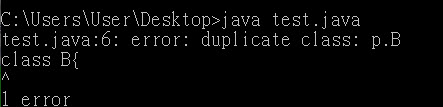
\includegraphics[width=85mm,scale=0.5]{SCN.jpg}}
\caption{\textbf{Compile error for using same class name after RcR}}
\label{fig:renameclassname}
\end{figure}

Also, this precondition is applicable even if the classes are defined in separate java files or any file is empty but are within the same folder. In Fig. \ref{fig:empty}, we try to apply RcR from \emph{A to C} or \emph{B to C} where C.java is an empty file, the compiler produces an error as shown in Fig. \ref{fig:efr}. 

\begin{figure}[th]
\centering
\begin{minipage}[t]{0.45\linewidth}
\begin{lstlisting}[language=java, basicstyle=\scriptsize\ttfamily,frame=single]
A.java

public class A{
}
	
class B{
}


C.java
//empty file
 
\end{lstlisting}
\centering(a) Before
\end{minipage}
\hfill
\begin{minipage}[t]{0.45\linewidth}
\begin{lstlisting}[language=java, basicstyle=\scriptsize\ttfamily,frame=single]
A.java

public class A{
}
	
class C{
}


C.java
//empty file

\end{lstlisting}
\centering(b) After
\end{minipage}
\caption{\textbf{RcR from B to C even if C.java is empty}}
\label{fig:empty}
\end{figure}

\begin{figure}[H]
\centerline{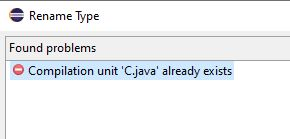
\includegraphics[width=85mm,scale=0.5]{EFE.jpg}}
\caption{\textbf{Compile error for same file name after RcR}}
\label{fig:efr}
\end{figure}


Furthermore, the same situation occurs in nested classes. The examples below show that for RcR we can not use the same name either as inner or as outer class for nested classes like Fig. \ref{fig:original}.

\begin{figure}[th]
\centering
\begin{minipage}[t]{0.5\linewidth}
\begin{lstlisting}[language=java, basicstyle=\scriptsize\ttfamily,frame=single]
package p;

public class A{	

  class M{
  }

  class N{
  }
} 
\end{lstlisting}
\end{minipage}
\caption{\textbf{Nested Class before RcR}}
\label{fig:original}
\end{figure}

\textbf{Example 1:} In order to implement RcR for inner class, we should pre-check that we do not use the same name as any of other inner class name. From Fig. \ref{fig:nestedclass1}, when we try to rename refactor the inner class from M to N, the Java compiler produces an error as shown in Fig. \ref{fig:NC1}.

\begin{figure}[th]
\centering
\begin{minipage}[t]{0.5\linewidth}
\begin{lstlisting}[language=java, basicstyle=\scriptsize\ttfamily,frame=single]
package p;

public class A{	
    
  class N{
  }
    
  class N{
  }
} 
\end{lstlisting}
\end{minipage}
\caption{\textbf{Example 1 for Nested Class after RcR from M to N}}
\label{fig:nestedclass1}
\end{figure}

\begin{figure}[H]
\centerline{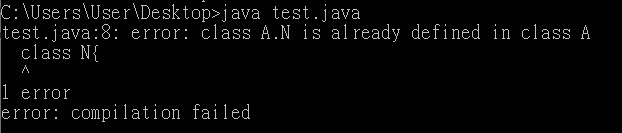
\includegraphics[width=75mm,scale=0.4]{NC1.jpg}}
\caption{\textbf{Compile error for duplicate inner class name after RcR}}
\label{fig:NC1}
\end{figure}

\textbf{Example 2:} In order to implement RcR for outer class, we should pre-check that we do not use the same name as any of the inner class name and vice-versa. From Fig. \ref{fig:nestedclass2}, when we try to use same name for outer class and inner class, the Java compiler produces an error as shown in Fig. \ref{fig:NC2} and Fig. \ref{fig:NC3}.

\begin{figure}[th]
\centering
\begin{minipage}[t]{0.45\linewidth}
\begin{lstlisting}[language=java, basicstyle=\scriptsize\ttfamily,frame=single]
package p;

public class M{	
  
  class M{
  }
	
  class N{
  }
} 
\end{lstlisting}
\centering{(a) After RcR on Outer Class A to M}
\end{minipage}
\hfill
\begin{minipage}[t]{0.45\linewidth}
\begin{lstlisting}[language=java, basicstyle=\scriptsize\ttfamily,frame=single]
package p;

public class A{	
    
  class A{
  }
    
  class N{
  }
} 
\end{lstlisting}
\centering{(b) After RcR on Inner Class N to A}
\end{minipage}
\caption{\textbf{Example 2 of Nested Class after RcR}}
\label{fig:nestedclass2}
\end{figure}

\begin{figure}[H]
\centerline{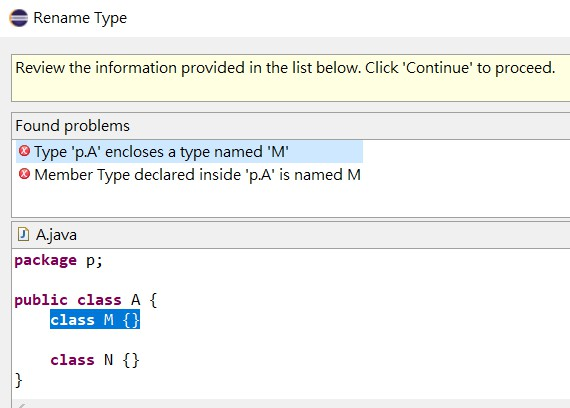
\includegraphics[width=75mm,scale=0.4]{NC2.jpg}}
\caption{\textbf{Compile error for RcR outer class same as inner class name}}
\label{fig:NC2}
\end{figure}

\begin{figure}[H]
\centerline{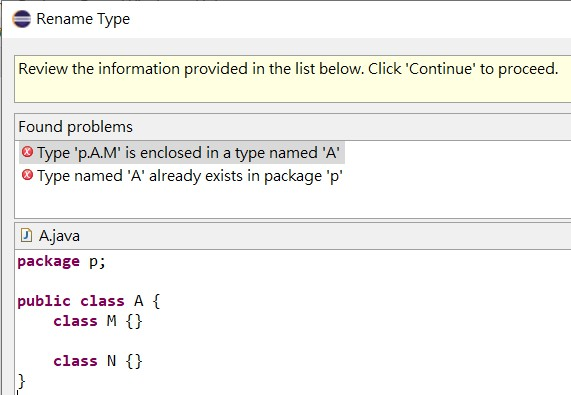
\includegraphics[width=75mm,scale=0.4]{NC3.jpg}}
\caption{\textbf{Compile error for RcR inner class same as outer class name}}
\label{fig:NC3}
\end{figure}

Therefore, checking whether a class with the same name already exists in a package should be the first precondition for RcR. 
   
